\subsection{Use Cases}
\label{sec:usecases}

\begin{figure}[htb]
	\centering
	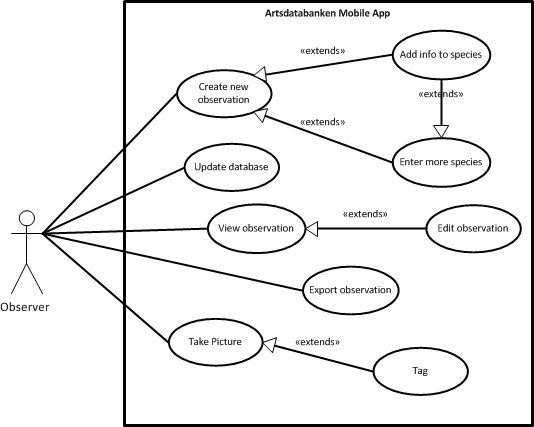
\includegraphics[width=0.9\textwidth]{reqspec/mainusecase.jpg}
	%\caption{Use Case Diagram}
	\label{fig:usecase}
\end{figure}

In the following use cases, there is only one actor: the generic user
\hspace{2em}

\begin{tabular}[t]{|l|p{0.8\textwidth}|}
	\multicolumn{2}{c}{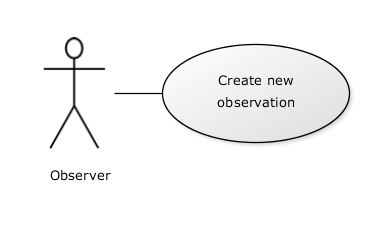
\includegraphics[width=0.8\textwidth]{reqspec/uc/cno.png}}\\\hline
	Use Case 1&Create New Observation\\\hline
	Requirement(s)&F1\\\hline
	Preconditions&User wants to register an observation\\\hline
	Flow&1. User taps the new observation button\newline
	2. User selects a species type (bird, bug, etc.)\newline
	3. User selects location from list of close locations, or selects GPS location\newline
	4. User adds one species. Helped by auto-complete\newline
	5. User saves the observation.\\\hline
	Extensions& 1a. Add number observed to species\newline
	4a. Add more info to the species, see Use Case 2\newline
	4b. Add more species into observation, see Use Case 3\\\hline
	Postconditions&A new observation has been saved and the user is directed back to the main menu.\\\hline
	Complexity&Medium\\\hline
	Priority&High\\\hline
\end{tabular}

\hspace{4em}

\begin{tabular}[t]{|l|p{0.8\textwidth}|}
	\multicolumn{2}{c}{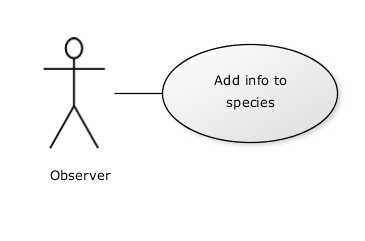
\includegraphics[width=0.8\textwidth]{reqspec/uc/addinfo.png}}\\\hline
	Use Case 2&Add More Information to Species\\\hline
	Requirement(s)&F2\\\hline
	Preconditions&User wants to specify more details about an observation\\\hline
	Flow& 1. User taps the the species row to bring up the new detail window.\newline
	2. User selects additional info to enter from such categories as \newline
	Activity (drop down?) \newline
	Age\newline
	Sex\newline
	Start Date\newline
	Start Time\newline
	End date \newline
	End Time \newline
	Comment \newline
	Picture \newline
	%	\begin{itemize}
	%		\item Activity (drop down?)
	%		\item age
	%		\item sex
	%		\item date
	%		\item time
	%		\item enddate
	%		\item endtime	
	%		\item comment
	%		\item picture
	%\end{itemize}
	3. User taps OK to get back to the main observation window.\\\hline
	Extensions& \\\hline
	Postconditions& Additional information about an observation has been saved.\\\hline
	Complexity&Low\\\hline
	Priority&High\\\hline
\end{tabular}

\hspace{2em}


\begin{tabular}[t]{|l|p{0.8\textwidth}|}
	\multicolumn{2}{c}{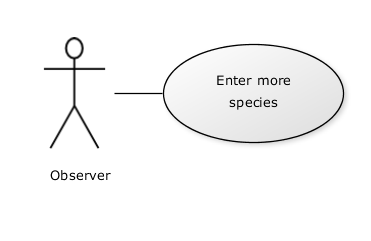
\includegraphics[width=0.8\textwidth]{reqspec/uc/entermore.png}}\\\hline
	Use Case 3&Add another species to observation\\\hline
	Requirement(s)&F3\\\hline
	Preconditions&User wants to add another species to the observation\\\hline
	Flow&1. User taps 'Add species' button.\newline
	2. Optionally selects another location, otherwise the same one is selected.\newline
	3. User selects species helped by auto complete. \newline
	4. User taps 'OK' to go back to main observation window \\\hline
	Extensions& \\\hline
	Postconditions& Additional species has been added to the observation\\\hline
	Complexity&Low\\\hline
	Priority&High\\\hline
\end{tabular}

\hspace{2em}


\begin{tabular}[t]{|l|p{0.8\textwidth}|}
	\multicolumn{2}{c}{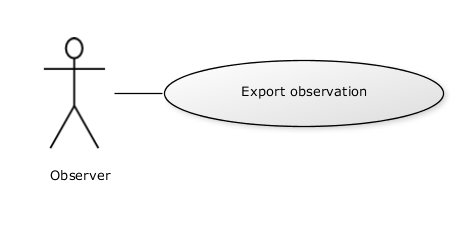
\includegraphics[width=0.8\textwidth]{reqspec/uc/export.png}}\\\hline
	Use Case 4&Export  observations\\\hline
	Requirement(s)&F4\\\hline
	Preconditions& User wants to export their observations \\\hline
	Flow&1. User taps the 'Export' button on the main screen\newline
	2. User selects the observations to be exported\newline
	3. User taps the export button\\\hline
	Extensions& \\\hline
	Postconditions&Observations are exported in excel or XML format to the user's email so they can be imported into the online system later\\\hline
	Complexity&High\\\hline
	Priority&Medium\\\hline
\end{tabular}

\hspace{2em}


\begin{tabular}[t]{|l|p{0.8\textwidth}|}
	\multicolumn{2}{c}{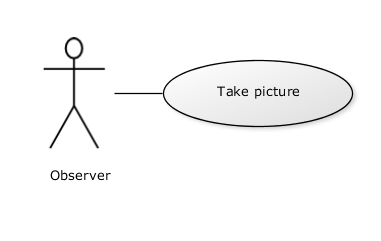
\includegraphics[width=0.8\textwidth]{reqspec/uc/takepicture.png}}\\\hline
	Use Case 5&Take picture\\\hline
	Requirement(s)&F5\\\hline
	Preconditions&User wants to take a picture to be attached to an observation\newline
	The device has a camera\\\hline
	Flow&1. User taps 'Take picture' button.\newline
	2. User takes picture \\\hline
	Extensions& 2a. User adds a description to the picture\\\hline
	Postconditions&Picture is stored on the phone with an easily recognizable filename so it can be attached to an observation 	later\\\hline
	Complexity&Medium\\\hline
	Priority&Low\\\hline
\end{tabular}
	
\hspace{2em}


\begin{tabular}[t]{|l|p{0.8\textwidth}|}
	\multicolumn{2}{c}{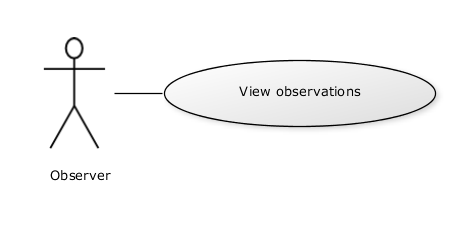
\includegraphics[width=0.8\textwidth]{reqspec/uc/viewobs.png}}\\\hline
	Use Case 6&View observations\\\hline
	Requirement(s)&F6\\\hline
	Preconditions&User wants to view locally stored observations\\\hline
	Flow&1. User taps the 'View observations' button.\newline
	2. User selects the observation from a list of stored observations \\\hline
	Extensions&None \\\hline
	Postconditions&None\\\hline
	Complexity&Medium\\\hline
	Priority&Low\\\hline
\end{tabular}

\hspace{2em}


\begin{tabular}[t]{|l|p{0.8\textwidth}|}
	\multicolumn{2}{c}{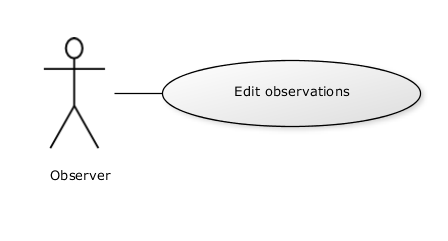
\includegraphics[width=0.8\textwidth]{reqspec/uc/editobs.png}}\\\hline
	Use Case 7&Edit observations\\\hline
	Requirement(s)&F7\\\hline
	Preconditions&User wants to edit a previously created observations\newline
	There exists previously made observations\\\hline
	Flow&1. User taps the 'View observations' button.\newline
	2. User selects the observation from a list of stored observations\newline
	3. User taps the 'Edit' button \newline
	4. User makes desired changes and/or additions\newline
	5. User taps save button\\\hline
	Extensions& \\\hline
	Postconditions&Changes are stored on the device\\\hline
	Complexity&Low\\\hline
	Priority&Low\\\hline
\end{tabular}

\hspace{2em}


\begin{tabular}[t]{|l|p{0.8\textwidth}|}
	\multicolumn{2}{c}{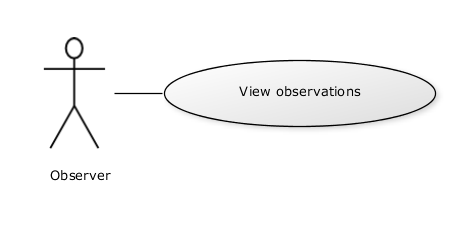
\includegraphics[width=0.8\textwidth]{reqspec/uc/viewobs.png}}\\\hline
	Use Case 8&Update Database\\\hline
	Requirement(s)&F8\\\hline
	Preconditions&User wants to update the database because new species or
	locations have been added to the website\\\hline
	Flow&1. User taps options button\newline
	2. User selects the option to update the database\\\hline
	Extensions& \\\hline
	Postconditions&New Species and locations are stored on the phone to help
	the user with auto-complete and correctly choose locations for observations.\\\hline
	Complexity&Medium\\\hline
	Priority&Low\\\hline
\end{tabular}
